\Chapter{Az alkalmazás specifikációja}

\Section{Általános leírás}

A dolgozat célja egy olyan alkalmazás elkészítése, amely különböző feladatok időbeli ütemezésével foglalkozik. Az alkalmazás egy 8 órás időegységen belül vizsgálja, hogy a feladatok prioritása és a feladatokra szánt időtartamok megadásával hogyan lehet adott szempontrendszer alapján optimális, vagy ahhoz közeli ütemezést elérni. Figyelembe veszi a maximum időkeretet, így az elhanyagolható tevékenységeket kiszelektálja és a hatékonyabb időbeosztás elérését szolgáló tevékenységek beütemezését valósítja meg. A különböző feladatokat adataikkal együtt a hozzáadás sorrendjében vizuálisan ábrázolja, végül pedig egy ütemezett eredményt jelenít meg a grafikus felületen, azokkal az elemekkel, amelyek belefértek az adott időkeretbe az adott követelményrendszer szerint.

\Section{Feladatok}

A feladatok definiálása az egyik alapvető funkciója az alkalmazásnak, hiszen el kell tárolni a hozzá tartozó adatokkal együtt, hogy aztán eszerint az ütemezést végre lehessen hajtani. 

\SubSection{Feladatokhoz tartozó adatok}

Egy adott tevékenység meghatározásakor szükséges megadni a tevékenység nevét, a prioritását, ami jelzi, hogy mennyire fontos egy adott feladattal mihamarabb végezni, valamint azt az időtartamot, amely előreláthatólag lefedi a tevékenység hosszát.

Cím (TaskTitle): A feladat neve, a közeljövőben végrehajtani kívánt tevékenység egy szóval ábrázolva, pl.: bevásárlás.

Prioritás (TaskPriority): A prioritás megadásánál 3 lehetőség közül lehet választani. 1-től 3-ig adható meg, mennyire tartja fontosnak a felhasználó a feladat elvégzését; minél magasabb számérték megadása történik, annál fontosabbként lesz kezelve az adott feladat. Tehát, az 1-es számérték jelzi az alacsony prioritást, a 2-es számérték jelzi a közepes prioritást, a 3-as számérték pedig a magas prioritást. Prioritások használatakor bevett szokás szín szerinti megkülönböztető jelzést használni, így ebben az alkalmazásban is sor kerül erre. A megjelenítés során a diagramsáv keretének színe jelzi, hogy az adott feladathoz milyen értéket rendeltünk. Magas prioritás esetén piros, közepes esetén szürke, alacsony prioritás esetén zöld kerettel jelenik meg a grafikusan ábrázolt feladat sávja.

Időtartam (TaskDuration): A feladatokra szánt időtartamoknak a percben való megadására van lehetőség, mivel ezáltal a rövidebb, pár perces tevékenységek ugyanolyan könnyedén megadhatóak, mint a hosszabb, akár 1-2 órásak is. Mivel az ütemezés 8 órás időegységen belül történik, ezért 8 óránál, azaz 480 percnél hosszabb időtartamú esemény megadására nincs lehetőség, mivel annak beütemezésére úgysem kerülne sor.

Hasonló alkalmazásoknál megfigyelhető, hogy egy feladathoz még számos egyéb adat hozzárendelése lehetséges, például:

\begin{itemize}
	\item leírás,
	\item színjelzés,
	\item létrehozás ideje,
	\item különböző címkék csoportosításhoz,
	\item tulajdonos,
	\item csapattagok,
	\item státusz jelzés.
\end{itemize}

Ezeknél az alkalmazásoknál gyakran megfigyelhető, hogy nem feltétlen egy felhasználó számára készített programokról van szó, hanem lehetőséget nyújtanak több felhasználó számára, hogy például egy adott projektet egyidejűleg elérjenek és közösen dolgozzanak rajta. A felsorolt adatok pedig segítenek nyomon követni és átláthatóbbá tenni a csapatmunkát.

A programomban azért a prioritásokra és időtartamokra fókuszálok, mert az előző fejezetben nyilvánvalóvá vált, hogy ez a két tényező a legtöbb hatékonyságnövelő módszer alapja, ezáltal ez tűnt célszerűnek. A későbbiekben, amennyiben lehetőségem nyílik rá, megfontolandónak tartom egyéb tényezők figyelembevételét is, azaz, hogy hogyan tudnám súlyozni a feladatokat különböző szempontok szerint az előzőek mellett, mint például mennyire nehéz vagy épp mennyi haszonnal jár az elvégzése számunkra. 

\SubSection{Feladatok hozzáadása}

Feladat hozzáadásakor a cím, a prioritás, és a feladatra szánt becsült időtartam megadása kötelező (3.1. ábra), a három adat közül bármely kihagyása esetén egy felugró üzenet figyelmeztet a hibás érték(ek)re. Azonos nevű feladat hozzáadása nem lehetséges. Az időtartamhoz maximum 480 perc megadása áll rendelkezésre, erre fel is hívja a figyelmet egy üzenet a kurzort az időtartam felé mozgatva. A prioritásnál szintén hasonló üzenet jelzi a megadható prioritásértékeket (1-alacsony, 2-közepes, 3-magas).

\begin{figure}[h]
	\centering
	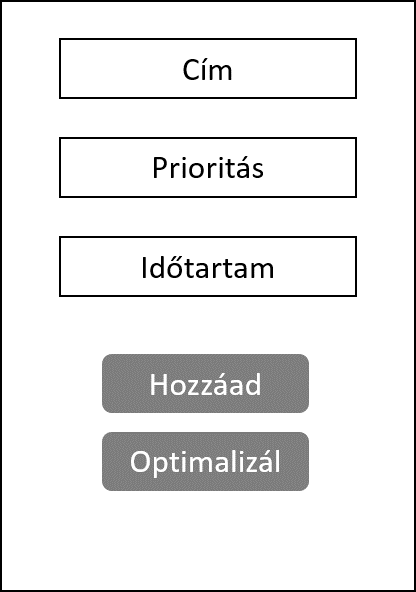
\includegraphics[scale=0.6]{images/addTasks.png}
	\caption{Feladatok definiálása a programban}
\end{figure}

Megfelelő adatok megadása esetén, a „Hozzáad” gombra kattintva egy felugró üzenet jelzi, hogy a feladat hozzáadása sikeres volt. Ezzel egyidejűleg a feladat grafikus ábrázolása is megtörténik a diagramon. Láthatóvá kell tenni a feladat címét, mögötte a hozzá tartozó időtartammal, valamint egy, az időtartammal megegyező hosszúságú sávot, a prioritásnak megfelelő piros, szürke vagy zöld kerettel.(3.2. ábra)

\begin{figure}[h]
	\centering
	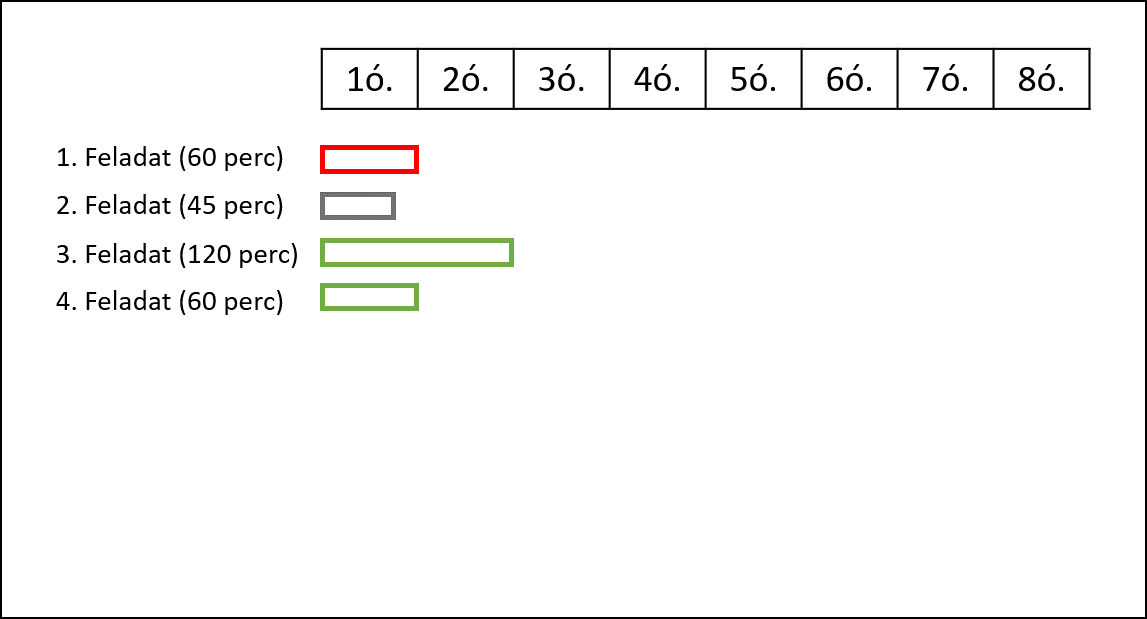
\includegraphics[scale=0.8]{images/diagram.png}
	\caption{Feladatok grafikus ábrázolása}
\end{figure}

Következő feladatok definiálásakor a diagramon megjelenő információk mindig az előzőek alá kerülnek.

\Section{Optimalizálás és ütemezés}

Az alkalmazás lényegi funkciója. A feladatok ütemezése során a programnak az időkeretbe beleférő legnagyobb összértéket kell előállítania, ezáltal pedig a lehető leghatékonyabb megoldást, tervezetet megkapni. Az ütemezés kivitelezésére külön fejezetben kerül sor, ahol meghatározom magát az ütemezési problémát, valamint a lehetséges megoldásokat rá. Az optimalizálás a program futása során nem automatikusan történik, minden egyes újabb feladat hozzáadásakor, hanem a felhasználó az általa szükségesnek vélt feladatok hozzáadása után kérheti az ütemezést az "Optimalizál" gomb megnyomásával.

Az optimalizálás végrehajtásához minimum két feladat megléte szükséges. Az "Optimalizál" gomb megnyomására a program végrehajtja az optimalizálást és az ütemezést. A sikeres ütemterv létrehozását egy felugró ablak jelzi. Ezután megjelenik egy "Ütemezett sorrend" felirat, melyet követően azon feladatok nevei szerepelnek, amelyeket a program beütemezett a 8 órás időkeretbe, olyan sorrendben, ahogy azokat célszerű végrehajtani az ütemező szerint. Az ütemterv grafikus ábrázolása során a diagramon megjelenő sávok egymás mellett jelennek meg lehetőség szerint kitöltve a 8 órányi időtartamot. Az ütemező a kihagyott feladatok neveit is megjeleníti. (3.3. ábra) Ha az ütemezendő feladatok összideje nem éri el a 8 órát, ezáltal minden elem sikeresen belekerült az időkeretbe, akkor ezt egy "Minden feladat belefért az időkeretbe!" felirat jelzi.

\begin{figure}[h]
	\centering
	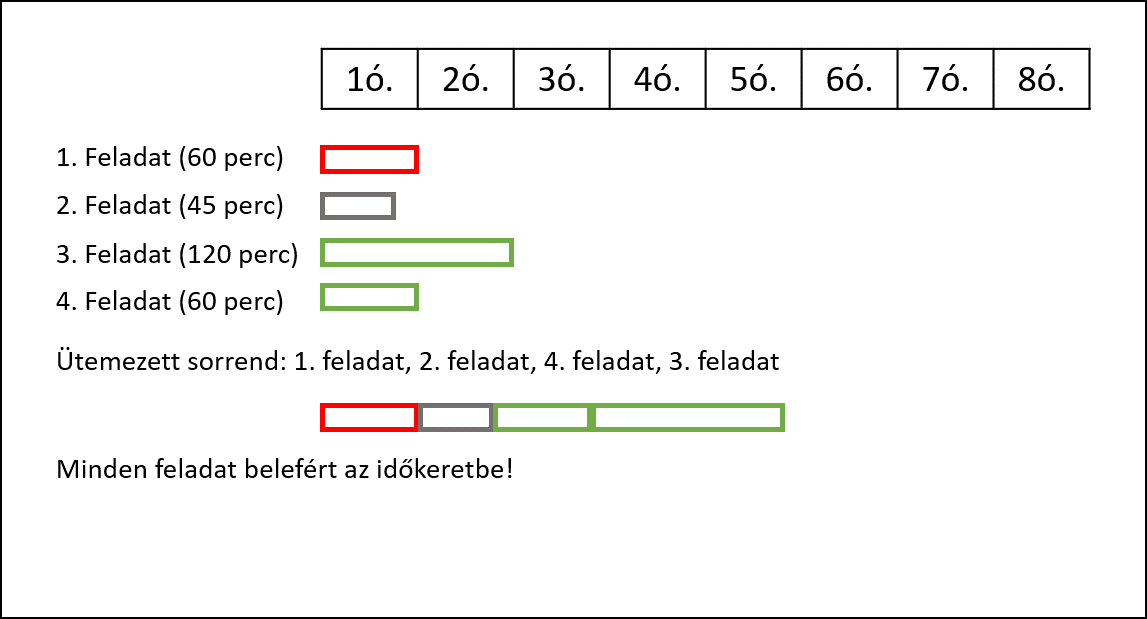
\includegraphics[scale=0.8]{images/scheduledTasks.png}
	\caption{Ütemterv grafikus ábrázolása}
\end{figure}
